
It originates in \fullcite{scvo85} (1985). 

\begin{center}
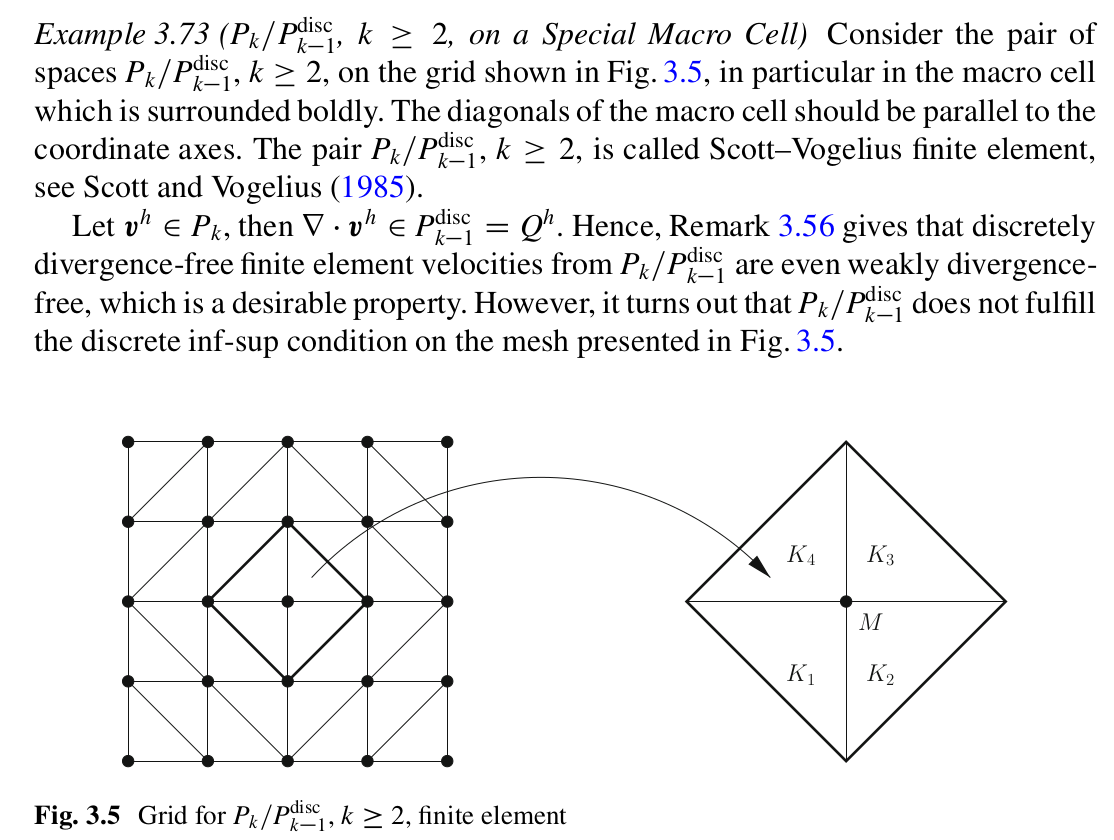
\includegraphics[width=10cm]{images/pair_scott_vogelius/john_scott_vogelius}\\
\captionfont{Taken from John \cite[p70]{john16}.} 
\end{center}

See also \textcite{jolm17} (2017) in which the P2P1, SV (P2P-1), Bernardi-Raugel, and P2+P-1 elements 
are compared for a thermo-mechanically driven convection problem in a triangle (see \stone~51, 
although I use the P1+P1 element in this stone).
 
In Chapter 9 of \textcite{bobm13} we find: 
``
We also remark that the discontinuous
pressure version of the Hood–Taylor element typically
results in an unstable method. However, stability can be
recovered by imposing certain restrictions on the mesh for
$k \ge 3$ (see Vogelius, 1983; \cite{scvo85}), or
by taking advantage of suitable stabilization procedures for
$k\ge 1$ (see Mansfield, 1982; Boffi, 1995).
''

In \textcite{fams21} we find:
``The Scott-Vogelius element is given by choosing continuous piecewise polynomials of degree $k$ for
the velocity and discontinuous piecewise polynomials of degree $k-1$ for the pressure. While this clearly
implies that $\nabla\cdot V_h \in Q_h$, inf-sup stability of the Scott–Vogelius element 
is more delicate, and is a topic of ongoing research. 
In two dimensions, Scott \& Vogelius proved \cite{scvo85} that the element is inf-sup
stable for $k\ge 4$ if the mesh does not have nearly singular vertices. 
In three dimensions, it was proven more recently in [67] that the element is stable 
for $k\ge 6$ on uniform meshes. The stability on general
tetrahedral meshes continues to be an open question.

On barycentrically refined meshes, however, the pair is known to be stable for polynomial order
$k = d$, see [48, Section 4.6] for the 2D case and [65] for the 3D case. If one is willing to 
consider the more complicated Powell–Sabin split, the order can be reduced further to 
$k = d-1$ [66, 68]. The two
refinement patterns are shown for the two dimensional case in Figure 1. In this work we will consider
the case of $k \ge d$ on barycentrically refined meshes, but the arguments apply mutatis mutandis to the
Powell–Sabin split.
''

\begin{center}
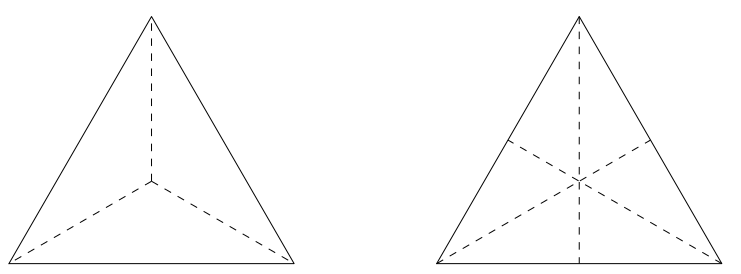
\includegraphics[width=8cm]{images/pair_scott_vogelius/scottvogelius_split}\\
{\captionfont 
Barycentrically refined triangle (also known as Alfeld split) on the left,
and Powell–Sabin split on the right. Taken from \textcite{fams21} (2021).}
\end{center}

